\section{Varying Length Pattern Classification for Real World Data}


Dataset 2B consists of image histogram data pertaining to five class labels in which each image is represented by a set of 36, 23 dimensional vectors, i.e each image is represented by $36x23$ matrix. In the training phase each of row from the image matrices are treated as separate examples with the
same label as the parent image. In the classification phase, the classification of each image involves the calculating of the conditional probability that the image belongs to the class i as the product of the individual conditional probabilities of its constituent rows, i.e for an image matrix X and class label i.

 \begin{align*}
      p(y=y_i) &= \prod_{n=1}^{n} p(y=y_i) \\
                    &= \prod_{j=1}^{N}\sum_{k=1}^{K}w_{ik}. \mathcal{N}(x_n|\mu_{ik},c_{ik})
  \end{align*}
  

In both cases, the optimal model was found to be the cluster combination of [8,8,8,8,8] and a thorough search through the combination parameters were not feasible as the training of the model is computationally expensive across 150,000 data points

% -----------------------------------------------------------
{\rowcolors{3}{green!40!yellow!10}{green!0!yellow!30}
\begin{table}[!h]
\centering
\begin{tabular}{ |c|c|c|  }
\hline
\rowcolor{lightgray} Model & Training Accuracy & Val Accuracy \\
\hline
[1,1,1,1,1] & 23.13$\%$  & 22.88$\%$ \\   
 \hline
[2,2,2,2,2] & 45.77$\%$  & 47.17$\%$ \\ 
\hline
[3,3,3,3,3] & 57.62$\%$  & 47.45$\%$ \\
\hline
[4,4,4,4,4] & 61.85$\%$  & 51.97$\%$ \\
\hline
[5,5,5,5,5] & 67.37$\%$  & 61.58$\%$ \\
\hline
[6,6,6,6,6] & 69.64$\%$  & 62.42$\%$ \\
\hline
[7,7,7,7,7] & 70.21$\%$  & 66.10$\%$ \\
\hline
[8,8,8,8,8]  & 73.62 $\%$  & 66.66 $\%$ \\
\hline
\end{tabular}
\caption{Performance of models for Diagonal Covariance matrix}.
\label{table:9}
\end{table}
}

% -----------------------------------------------------------
{\rowcolors{3}{green!40!yellow!10}{green!0!yellow!30}
\begin{table}[!ht]
\centering
\begin{tabular}{ |c|c|c|  }
\hline
\rowcolor{lightgray} Model & Training Accuracy & Val Accuracy \\
\hline
[1,1,1,1,1] & 88.39$\%$  & 83.61$\%$ \\   
 \hline
[2,2,2,2,2] & 94.80$\%$  & 80.50$\%$ \\ 
\hline
[3,3,3,3,3] & 95.86$\%$  & 85.31$\%$ \\
\hline
[4,4,4,4,4] & 97.40$\%$  &  90.67 $\%$ \\
\hline
[5,5,5,5,5] & 98.86$\%$  & 94.63$\%$ \\
\hline
[6,6,6,6,6] & 99.02$\%$  & 94.63$\%$ \\
\hline
[7,7,7,7,7] & 99.26$\%$  & 94.35$\%$ \\
\hline
[8,8,8,8,8](optimal)  &  99.67 $\%$  & 95.19 $\%$ \\
\hline
\end{tabular}
\caption{Performance of models for Full Covariance matrix}.
\label{table:10}
\end{table}
}
\newpage




%------------------------------------------------------------
% \subsubsection*{Model Accuracy across combinations}

% \begin{figure}[!ht]
%     \centering
%     \begin{subfigure}[t]{0.5\textwidth}
%         \centering
%         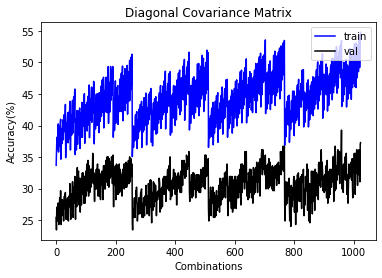
\includegraphics[height=2.5in]{Dataset_2a/diagonal covariance graph combinations.png}
%         \caption{Diagonal covariance combinations}
%     \end{subfigure}%
%     ~ 
%     \begin{subfigure}[t]{0.5\textwidth}
%         \centering
%         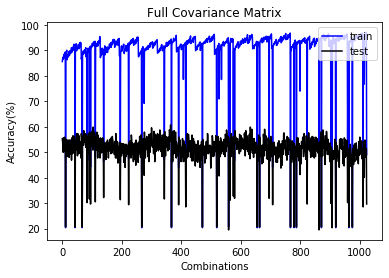
\includegraphics[height=2.5in]{Dataset_2a/full covariance graph combinations.png}
%         \caption{Full covariance combinations}
%     \end{subfigure}%
%     ~
%     \caption{Covariance Combinations}
%     \label{fig:23}
% \end{figure}


\begin{figure}[!h]
    \centering
    \begin{subfigure}[t]{0.5\textwidth}
        \centering
        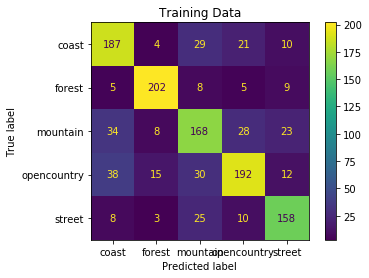
\includegraphics[height=2.5in]{Dataset_2b/diagonal covariance train confusion matrix.png}
        \caption{Train Data}
    \end{subfigure}%
    ~ 
    \begin{subfigure}[t]{0.5\textwidth}
        \centering
        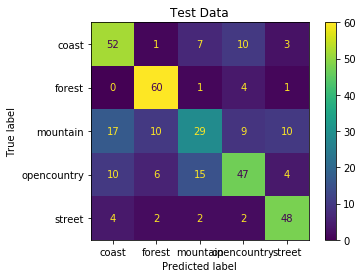
\includegraphics[height=2.5in]{Dataset_2b/diagonal covariance test confusion matrix.png}
        \caption{Validation Data}
    \end{subfigure}%
    ~
    \caption{Confusion Matrix for diagonal covariance}
    \label{fig:30}
\end{figure}

%------------------------------------------------------------
%\newpage

\begin{figure}[!h]
    \centering
    \begin{subfigure}[t]{0.5\textwidth}
        \centering
        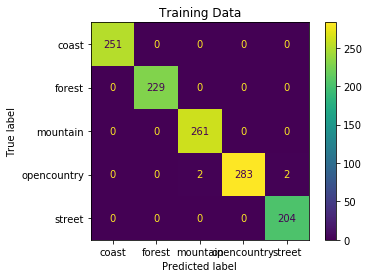
\includegraphics[height=2.5in]{Dataset_2b/full covariance train confusion matrix.png} 
        \caption{Train Data}
    \end{subfigure}%
    ~ 
    \begin{subfigure}[t]{0.5\textwidth}
        \centering
        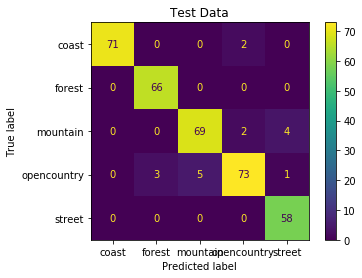
\includegraphics[height=2.5in]{Dataset_2b/full covariance test confusion matrix.png}
        \caption{Validation Data}
    \end{subfigure}%
    ~
    \caption{Confusion Matrix for full covariance}
    \label{fig:31}
\end{figure}


